\documentclass[conference]{IEEEtran}
\IEEEoverridecommandlockouts
% The preceding line is only needed to identify funding in the first footnote. If that is unneeded, please comment it out.
\usepackage{cite}
\usepackage{amsmath,amssymb,amsfonts}
\usepackage{algorithmic}
\usepackage{graphicx}
\graphicspath{{Imgs/}}
\usepackage{textcomp}
\usepackage{xcolor}
\usepackage{hyperref,graphicx}
\usepackage{multicol}
\usepackage{listings}
\usepackage{color}
\usepackage{float}
\lstloadlanguages{C,C++,csh,Java}

\definecolor{red}{rgb}{0.6,0,0} 
\definecolor{blue}{rgb}{0,0,0.6}
\definecolor{green}{rgb}{0,0.8,0}
\definecolor{cyan}{rgb}{0.0,0.6,0.6}

\lstset{
language=csh,
basicstyle=\footnotesize\ttfamily,
numbers=left,
numberstyle=\tiny,
numbersep=5pt,
tabsize=2,
extendedchars=true,
breaklines=true,
frame=b,
stringstyle=\color{blue}\ttfamily,
showspaces=false,
showtabs=false,
xleftmargin=17pt,
framexleftmargin=17pt,
framexrightmargin=5pt,
framexbottommargin=4pt,
commentstyle=\color{green},
morecomment=[l]{//}, %use comment-line-style!
morecomment=[s]{/*}{*/}, %for multiline comments
showstringspaces=false,
morekeywords={ abstract, event, new, struct,
as, explicit, null, switch,
base, extern, object, this,
bool, false, operator, throw,
break, finally, out, true,
byte, fixed, override, try,
case, float, params, typeof,
catch, for, private, uint,
char, foreach, protected, ulong,
checked, goto, public, unchecked,
class, if, readonly, unsafe,
const, implicit, ref, ushort,
continue, in, return, using,
decimal, int, sbyte, virtual,
default, interface, sealed, volatile,
delegate, internal, short, void,
do, is, sizeof, while,
double, lock, stackalloc,
else, long, static,
enum, namespace, string},
keywordstyle=\color{cyan},
identifierstyle=\color{red},
backgroundcolor=\color{cloudwhite},
}
\usepackage{caption}
\DeclareCaptionFont{white}{\color{white}}
\DeclareCaptionFormat{listing}{\colorbox{blue}{\parbox{\textwidth}{\hspace{15pt}#1#2#3}}}
\captionsetup[lstlisting]{format=listing,labelfont=white,textfont=white, singlelinecheck=false, margin=0pt, font={bf,footnotesize}}
\definecolor{cloudwhite}{rgb}{0.9412, 0.9608, 0.8471} 




\renewcommand{\abstractname}{Abstracto}
\def\BibTeX{{\rm B\kern-.05em{\sc i\kern-.025em b}\kern-.08em
    T\kern-.1667em\lower.7ex\hbox{E}\kern-.125emX}}
\begin{document}
\renewcommand\IEEEkeywordsname{Palabras clave}

{\footnotesize 
\title{Aplicación para calcular la entropía de bits en iOS y Android}
}

\author{
\IEEEauthorblockN{García García Jonathan Eduardo}
\IEEEauthorblockA{\href{mailto:jgarciag1404@alumno.ipn.mx}{jgarciag1404@alumno.ipn.mx}}
}

\maketitle

\begin{abstract}
Este documento es el reporte técnico, explicativo del proceso por el cúal se consiguio crear una aplicación que ejemplifique forma simple y didactica el calculo de la entropía de bits o entropía de Shannon
\end{abstract}


\section{Fundamento teórico}
En teória de la información, la 
\textbf{entropía }
de una variable aleatoria es el promedio de la "información", "sorpresa" o "incierta" inherente a los posibles resultados de la variable. El concepto the entropía de la información fue introducido por 
en su artículo de 1948 "A Mathematical Theory of Communication" y frecuentemente es llamada 
\textbf{entropía de Shannon }
en su honor. \\
Como ejemplo, considere una moneda con probabilidad p de caer en cara y probabilidad 1-p de caer en cruz.La entropía máxima es para p = 1/2, cuando no hay razón para esperar un resultado sobre otro, y en este caso, el lanzamiento de una moneda tiene una entropía de un bit. La entropía mínima es cuando p = 0 o p = 1, cuando el evento es conocido y la entropía es cero bits. Otros valores de p dan diferentes entropías entre cero y uno bits.
\\
\textbf{Fórmula:}\\

\begin{centering}
    $H(X)=-\sum{P(x_i)\log{P(x_i)}}_{i=1}^{n}$\\
\end{centering}

\textbf{Ejemplo.}\\
Dada una variable discreta aleatoria 
, con posibles resultados 
, que ocurren con probabilidad 
la entropía de 
esta formalmente definida como: 
donde Sigma denota la suma de los posibles valores de la variable y log es el logaritmo, la elección de la base varía entre las diferentes aplicaciones. La base 2 da la unidad de bits (o "shannons"), mientras que la base e da las "unidades naturales" nat, y la base 10 da una unidad llamada "dits", "bans" o "hartleys". 
\begin{figure}[h!]
    \centering
    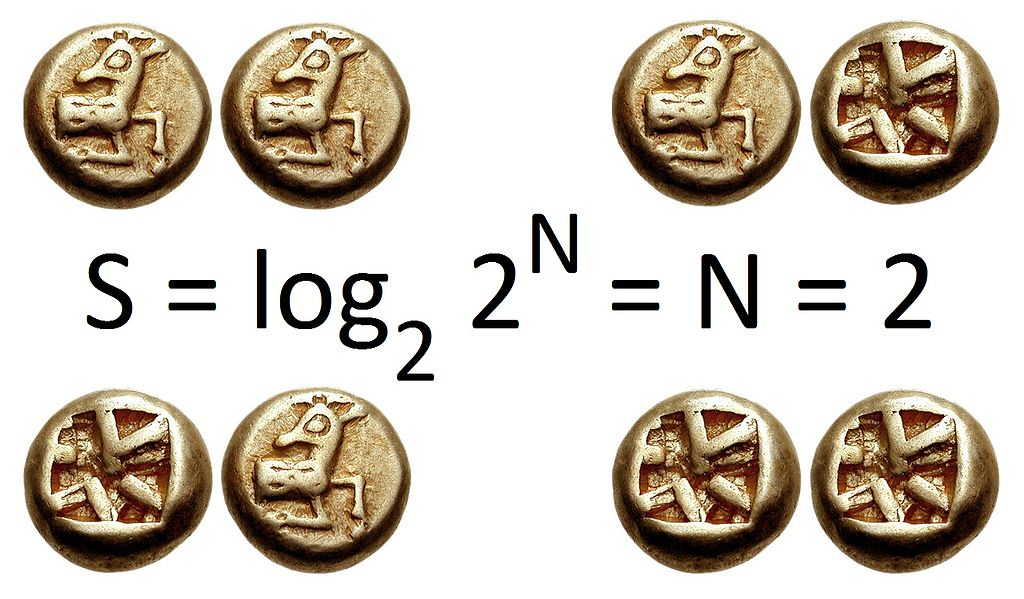
\includegraphics[width=7cm]{flip_coins.jpg}
\end{figure}


\section{Desarrollo}
\subsection{Plataformas:}
\begin{enumerate}
    \item iOS
    \item Android
\end{enumerate}
\subsection{Framework:}


\begin{figure}[h!]
    \centering
    
\includegraphics[width=7cm]{logox.png}
\end{figure}
Se opto por utilizar una tecnología de Desarrollo multiplataforma pues la interfaz es muy sencilla ademas de el poco tiempo de desarrollo y el deseo de abarcar dos plataformas donde y obtener exactamente el mismo resultado.\\
A pesar de esto se programarón funciones especificas siguiendo las reglas de cada plataforma como son:
\begin{itemize}
    \item Acceso a la camara
    \item Acceso a la galeria de fotos
    \item Acceso a el sistema de archivos
    \item Vinculación de librería nativa escrita en C++ para el cálculo rápido y eficiente de la entropía
\end{itemize}
\subsection{Calculando la entropía}
Se opto por crear una librería dinámica en el caso de Android y una librería estática para el caso de ios ambas escritas en C++
\begin{figure}[h!]
    \centering
    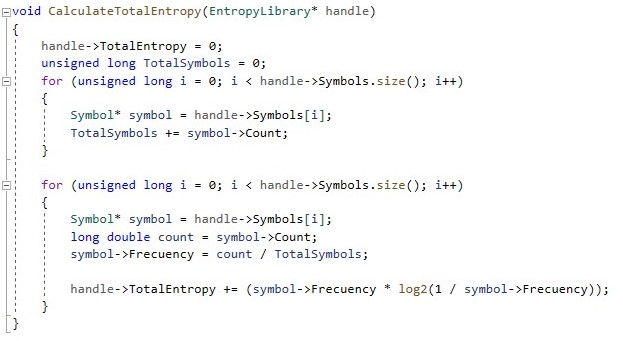
\includegraphics[width=9cm]{codeL.jpg}
\end{figure}
Este procedimiento es llamado desde el código de alto nivel para obtener el resultado de la entrópia y los simbolos, así como las probabilidades de cada uno mediante el uso de punteros.
\\Al final de el cálculo toda la memoria "insegura" es propiamente liberada.
\begin{figure}[h!]
    \centering
    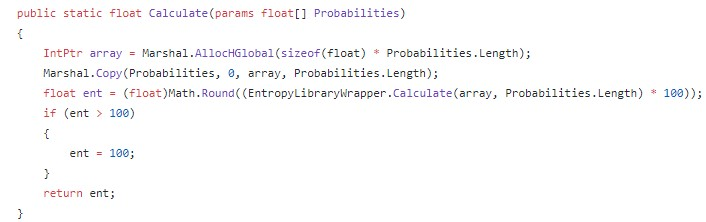
\includegraphics[width=9cm]{codeC.jpg}
\end{figure}
Igualmente se tiene acceso a una libreria gráfica para el calculo de histograma y entropía por imagen
\begin{figure}[h!]
    \centering
    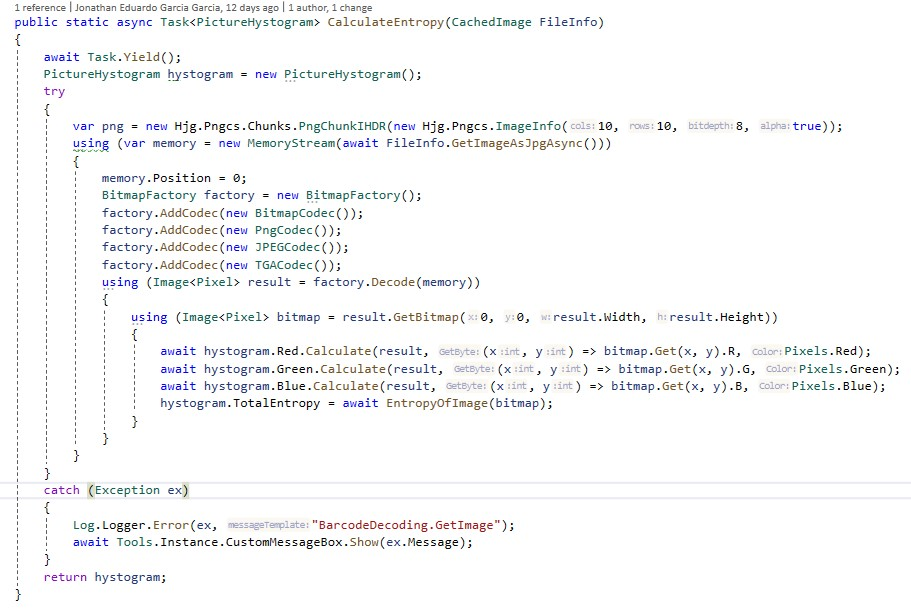
\includegraphics[width=9cm]{codeC2.jpg}
\end{figure}
\begin{figure}[h!]
    \centering
    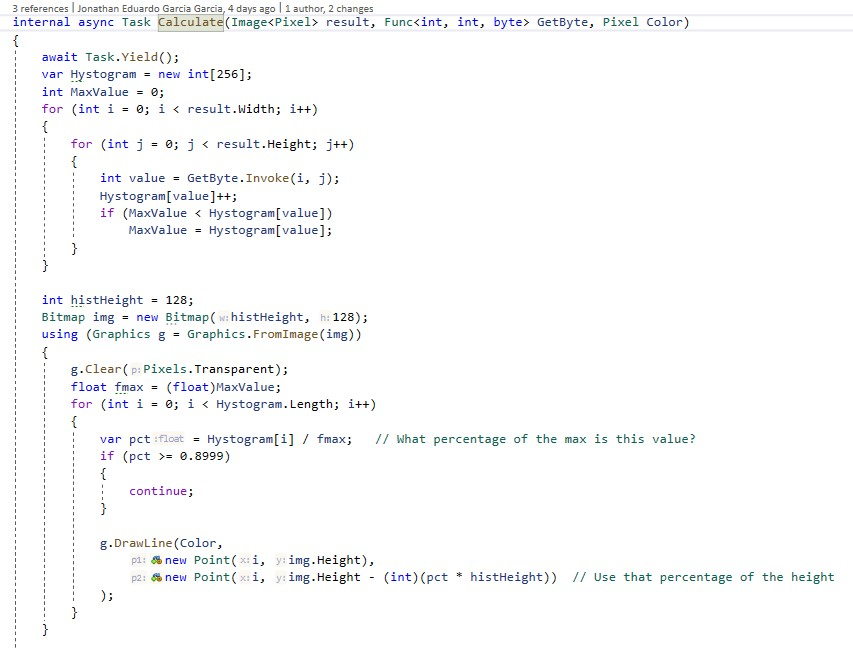
\includegraphics[width=9cm]{codeC3.jpg}
\end{figure}

\newpage
\subsection{Capturas de pantalla de código}


\begin{enumerate}
    \item Pantalla principal
    \begin{figure}[h!]
        \centering 
        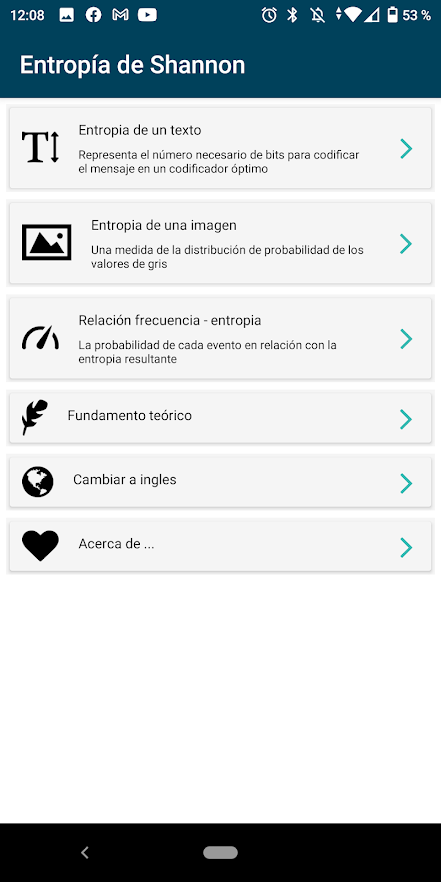
\includegraphics[scale=0.4]{captura0.png}
    \end{figure}
    \newpage  
    \item Pantalla para ingresar texto y calcular la entropía
    \begin{figure}[h!]
        \centering 
        
\includegraphics[scale=0.4]{captura2.png}
    \end{figure}
    \newpage  
    \item Resultados del de la entropía del texto
    \begin{figure}[h!]
        \centering 
        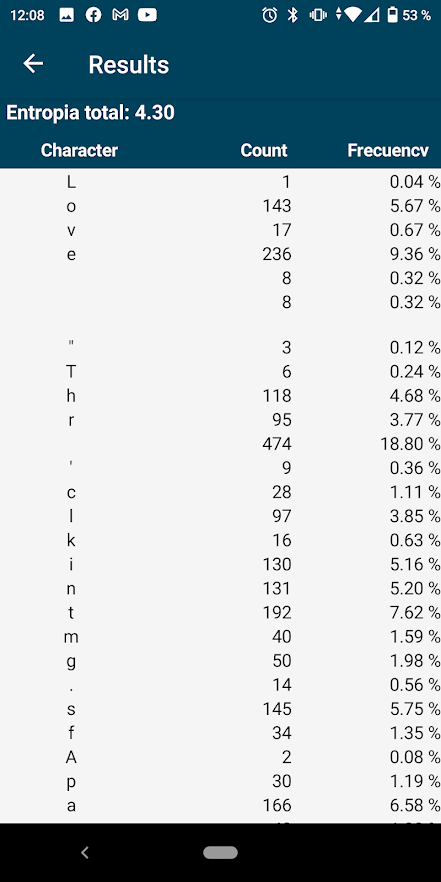
\includegraphics[scale=0.4]{captura4.png}
    \end{figure}
    \newpage  
    \item Entropía de una imagen
    \begin{figure}[h!]
        \centering 
        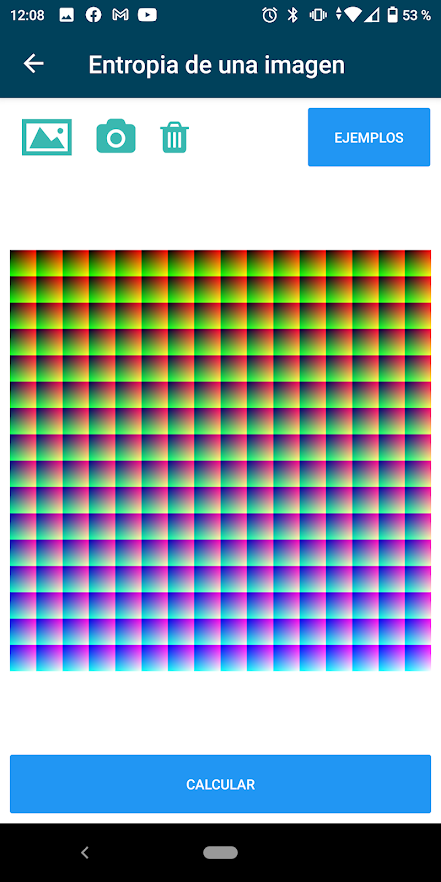
\includegraphics[scale=0.4]{captura3.png}
    \end{figure}
    \newpage  
    \item Resultados del de la entropía de una imagen
    \begin{figure}[h!]
        \centering 
        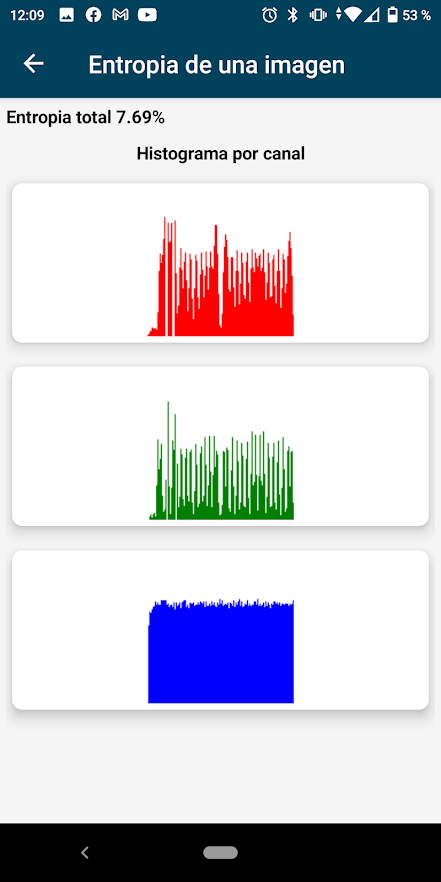
\includegraphics[scale=0.4]{captura1.png}
    \end{figure}
    \newpage  
    \item Fundamento teórico
    \begin{figure}[h!]
        \centering 
        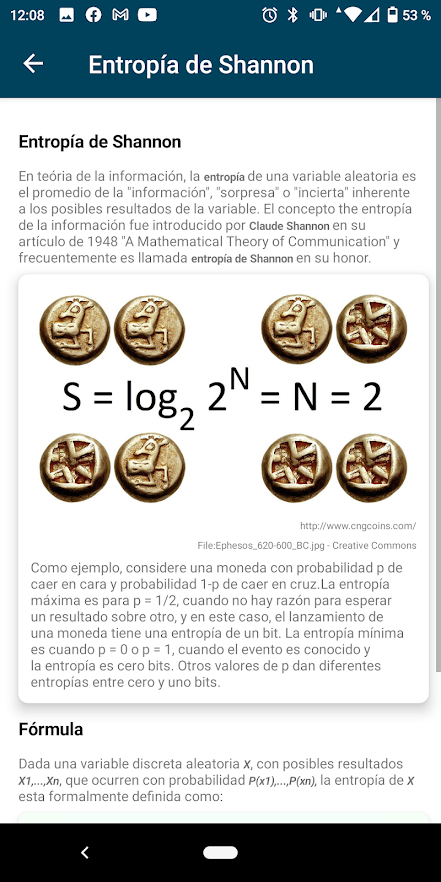
\includegraphics[scale=0.4]{captura5.png}
    \end{figure}
    \newpage  
    \item Relación entre la probabilidad de dos eventos y la entropía total
    \begin{figure}[h!]
        \centering 
        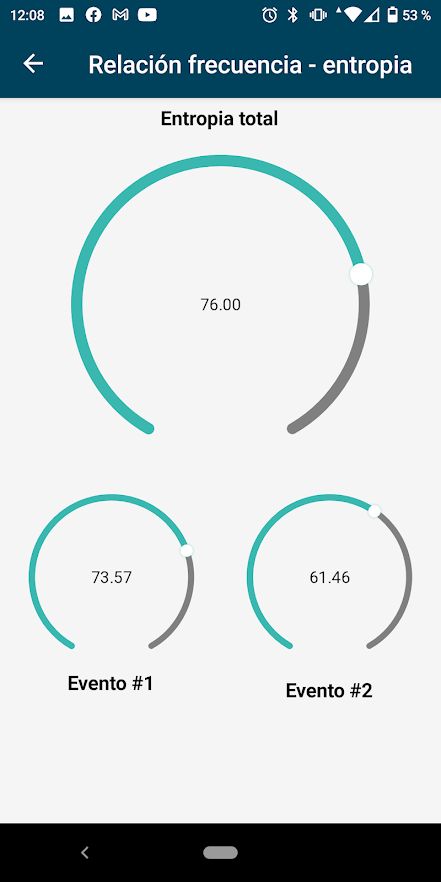
\includegraphics[scale=0.4]{captura6.png}
    \end{figure}
\end{enumerate}

\section{Disponible como "Shannon Entropy" en:}



\begin{center}
    \href{https://apps.apple.com/mx/app/shannon-entropy/id1566482675}
    {
        
\includegraphics{apple-app-store-badge.png}
    } 
\end{center}

\begin{center}
    \href{https://apps.apple.com/mx/app/shannon-entropy/id1566482675}{\underline{AppStore}}
\end{center}


\begin{center}
    
\includegraphics{google-play-badge.png}
\end{center}

\begin{center}
    \href{https://play.google.com/store/apps/details?id=com.jonathangg.shannonentropy}{\underline{PlayStore}}    
\end{center}


\begin{center}
    
\includegraphics[height=2cm]{github.png}
\end{center}
\begin{center}
    \href{https://play.google.com/store/apps/details?id=com.jonathangg.shannonentropy}{\underline{El código puede consultarse en Github}}    
\end{center}


\end{document}
